\documentclass[11pt]{utalcaDoc}
\usepackage{alltt}
\usepackage{underscore}
\usepackage[utf8]{inputenc}
\usepackage[activeacute,spanish]{babel}
\usepackage{verbatim}
\usepackage[pdftex]{graphicx}
\usepackage{ae}
\usepackage{amsmath}
\usepackage{amsfonts}
\usepackage{pdflscape}
\usepackage{inconsolata}
\usepackage{url}
\usepackage{hyperref}
\usepackage{listings}
\usepackage{tabularx}
\usepackage{makecell}
% \usepackage{placeins}
\usepackage[section]{placeins}
\usepackage[stable]{footmisc}
\usepackage{keyval}% http://ctan.org/pkg/keyval
\usepackage{minted}

\title{{\bf Seguridad Informática}\\ Proyecto 1}
\author{Erik Regla\\ eregla09@alumnos.utalca.cl}
\date{\today}



\newcommand{\informationResource}[9] {
    \begin{tabularx}{\linewidth}{|r|X|}
        \hline
        \textbf{Nombre}      & #1  \\ 
        \hline
        \textbf{Descripción} & #2  \\ 
        \hline
        \textbf{Categoría}   & #3  \\ 
        \hline
        \textbf{Ubicación}   & #4  \\ 
        \hline
        \textbf{Propietario} & #5  \\ 
        \hline
        \textbf{Valoración} &   Confidencialidad: #6 \\
                            &   Integridad: #7 \\
                            &   Disponibilidad: #8 \\
        \hline
        \textbf{Vulnerabilidades y Amenazas}  &  #9 \\ 
        \hline
    \end{tabularx}
}
    
    %% For offices
    \newcommand{\repetatOfficeInformationResource}[9]{
        \informationResource{#1\_001}{#2}{#3}{#4}{Jefe de #5}
        {#6}{#7}{#8}{#9}\\
    
        \informationResource{#1\_002}{#2}{#3}{#4}{Secretario de #5}
        {#6}{#7}{#8}{#9}\\
    
        \informationResource{#1\_003}{#2}{#3}{#4}{Ejecutivo de #5}
        {#6}{#7}{#8}{#9}
    }
    %% For depart
    \newcommand{\repeatDepartmentInformationResource}[9]{
        \informationResource{#1\_001}{#2}{#3}{#4}{Jefe de #5}
        {#6}{#7}{#8}{#9}\\
    
        \informationResource{#1\_002}{#2}{#3}{#4}{Secretario de #5}
        {#6}{#7}{#8}{#9}\\
    
        \informationResource{#1\_003}{#2}{#3}{#4}{Ejecutivo de #5}
        {#6}{#7}{#8}{#9}

        \informationResource{#1\_003}{#2}{#3}{#4}{Encargado de TI de #5}
        {#6}{#7}{#8}{#9}
    }

    %% For secretary
    \newcommand{\repeatSecretaryInformationResource}[9]{
        \informationResource{#1\_101}{#2}{#3}{#4}{Dirección de #5}
        {#6}{#7}{#8}{#9}\\

        \informationResource{#1\_101}{#2}{#3}{#4}{Secretario de #5}
        {#6}{#7}{#8}{#9}\\
    
        \informationResource{#1\_201}{#2}{#3}{#4}{Ejecutivo de #5}
        {#6}{#7}{#8}{#9}
    }
    

\newcommand{\repeatOnEachOfficeBase}[3]{
	\repetatOfficeInformationResource
	{NTB\_#1}
	{Thinkpad T490 series, equipo corporativo}
	{Hardware TI}
	{#2 - primer piso - recurso estático}
	{#2}
	{4}{5}{3}
	{
		\threatInformationBreach
		\threatResourceLost
		\threatHumanIntervention
		\threatRemoteIntervention
		\threatNaturalDisaster
		\threatHumanDisaster
	}

	\repetatOfficeInformationResource
	{EML\_#1}
	{Cuenta de correo corporativa}
	{Activo de información tangible}
	{EXE\_EXCHA\_001}
	{#2}
	{4}{5}{3}
	{
		\threatInformationBreach
		\threatRemoteIntervention
		\threatTransitive
	}

	\informationResource
	{NAS\_#1\_001}
	{Cisco NSS324 NAS, NAS local para equipo de la #2}
	{Hardware TI}
	{#2 - primer piso - recurso estático}
	{Departamento de TI - Encargado TI de #3}
	{4}{5}{3}
	{
		\threatCVE{CVE-2017-7494}{Ejecución remota de código}
		\threatInformationBreach
		\threatResourceLost
		\threatRemoteIntervention
		\threatNaturalDisaster
		\threatHumanDisaster
		\threatInterest
	}

	\informationResource
	{CAB\_#1\_001}
	{Armario de archivos para #2}
	{Infraestructura TI}
	{#2 - primer piso - recurso estático}
	{Jefe de #2}
	{5}{5}{5}
	{
		\threatNaturalDisaster
		\threatHumanDisaster
		\threatInterest
	}

	\informationResource
	{OFI\_#1\_001}
	{#2 - Instancia física}
	{Infraestructura TI}
	{#2 - primer piso - recurso estático}
	{Administración del edificio}
	{5}{5}{5}
	{
		\threatNaturalDisaster
		\threatHumanDisaster
	}

	\informationResource
	{RNG\_#1\_001}
	{Alarma de #2}
	{Control de entorno}
	{#2 - primer piso - recurso estático}
	{Administración del edificio}
	{5}{5}{5}
	{
		\threatHumanIntervention
		\threatRemoteIntervention
	}


	\informationResource
	{ARC\_#1\_001}
	{Archivo de #2 - registro de documentos}
	{Activos tangibles / Activos intangibles}
	{#2 - primer piso}
	{Jefe de #2}
	{5}{5}{4}
	{
		\threatNoPhysicalBackup
		\threatNoDigitalBackup
		\threatHumanIntervention
		\threatValue
	}
}
\newcommand{\repeatOnEachSecretaryBase}[3]{
	\repeatSecretaryInformationResource
	{NTB\_#1}
	{Thinkpad T490 series, equipo corporativo}
	{Hardware TI}
	{#2 - primer piso - recurso estático}
	{#2}
	{4}{5}{3}
	{
		\threatInformationBreach \\ &
		\threatResourceLost \\ &
		\threatHumanIntervention \\ &
		\threatNaturalDisaster \\ &
		\threatHumanDisaster
	}

	\repeatSecretaryInformationResource
	{EML\_#1}
	{Cuenta de correo corporativa}
	{Activo de información tangible}
	{EXE\_EXCHA\_001}
	{#2}
	{4}{5}{3}
	{
		\threatInformationBreach \\ &
		\threatHumanIntervention \\ &
		\threatTransitive \\ &
		\riskNameRolesNoDefinidos
		\riskNameQuiebreAutenticacionDeLlaveSeguridad \\ &
		\riskNameTransaccionRota \\ &
		\riskNamePhishing \\ &
	}

	\informationResource
	{NAS\_#1\_001}
	{Cisco NSS324 NAS, NAS local para equipo de la #2}
	{Hardware TI}
	{#2 - primer piso - recurso estático}
	{Departamento de TI - Encargado TI de #3}
	{4}{5}{3}
	{
		\threatCVE{CVE-2017-7494}{Ejecución remota de código} \\ &
		\threatInformationBreach \\ &
		\threatResourceLost \\ &
		\threatHumanIntervention \\ &
		\threatNaturalDisaster \\ &
		\threatHumanDisaster
	}

	\informationResource
	{CAB\_#1\_001}
	{Armario de archivos para #2}
	{Infraestructura TI}
	{#2 - primer piso - recurso estático}
	{Jefe de #2}
	{5}{5}{5}
	{
		\threatNaturalDisaster \\ &
		\threatHumanDisaster
	}

	\informationResource
	{OFI\_#1\_001}
	{#2 - Instancia física}
	{Infraestructura TI}
	{#2 - primer piso - recurso estático}
	{Administración del edificio}
	{5}{5}{5}
	{
		\threatNaturalDisaster \\ &
		\threatHumanDisaster
	}

	\informationResource
	{RNG\_#1\_001}
	{Alarma de #2}
	{Control de entorno}
	{#2 - primer piso - recurso estático}
	{Administración del edificio}
	{5}{5}{5}
	{
		\threatHumanIntervention
	}


	\informationResource
	{ARC\_#1\_001}
	{Archivo de #2 - registro de documentos}
	{Activos tangibles / Activos intangibles}
	{#2 - primer piso}
	{Jefe de #2}
	{5}{5}{4}
	{
		\threatNoPhysicalBackup \\ &
		\threatNoDigitalBackup \\ &
		\threatHumanIntervention
	}
}
\newcommand{\repeatOnEachDepartmentBase}[3]{
	\informationResource
	{SWI\_#1\_0001}
	{Switch general Cisco Catalyst 2960 para específico del departamento}
	{Hardware TI}
	{#2 - #3}
	{Departamento de TI - Encargado TI de #2}
	{1}{5}{5}
	{
		\threatCVE{CVE-2017-3881}{Ejecución arbitraria de código (resuelto)} \\ &
		\threatResourceLost \\ &
		\threatHumanIntervention \\ &
		\threatNaturalDisaster \\ &
		\threatHumanDisaster
	}


	\repeatDepartmentInformationResource
	{NTB\_#1}
	{Thinkpad T490 series, equipo corporativo}
	{Hardware TI}
	{#2 - #3 - recurso estático}
	{#2}
	{4}{5}{3}
	{
		\threatInformationBreach \\ &
		\threatResourceLost \\ &
		\threatHumanIntervention \\ &
		\threatNaturalDisaster \\ &
		\threatHumanDisaster
	}

	\repeatDepartmentInformationResource
	{EML\_#1}
	{Cuenta de correo corporativa}
	{Activo de información tangible}
	{EXE\_EXCHA\_001}
	{#2}
	{4}{5}{3}
	{
		\threatInformationBreach \\ &
		\threatHumanIntervention \\ &
		\threatTransitive \\ &
		\riskNameRolesNoDefinidos
		\riskNameQuiebreAutenticacionDeLlaveSeguridad \\ &
		\riskNameTransaccionRota \\ &
		\riskNamePhishing \\ &
	}

	\informationResource
	{NAS\_#1\_001}
	{Cisco NSS324 NAS, NAS local para equipo de la #2}
	{Hardware TI}
	{#2 - #3 - recurso estático}
	{Departamento de TI - Encargado TI de #2}
	{4}{5}{3}
	{
		\threatCVE{CVE-2017-7494}{Ejecución remota de código} \\ &
		\threatInformationBreach \\ &
		\threatResourceLost \\ &
		\threatHumanIntervention \\ &
		\threatNaturalDisaster \\ &
		\threatHumanDisaster
	}

	\informationResource
	{CAB\_#1\_001}
	{Armario de archivos para #2}
	{Infraestructura TI}
	{#2 - #3 - recurso estático}
	{Jefe de #2}
	{5}{5}{5}
	{
		\threatNaturalDisaster \\ &
		\threatHumanDisaster \\ &
		\riskNameRecuperacionDesastres
	}

	\informationResource
	{OFI\_#1\_001}
	{#2 - Instancia física}
	{Infraestructura TI}
	{#2 - #3 - recurso estático}
	{Administración del edificio}
	{5}{5}{5}
	{
		\threatNaturalDisaster \\ &
		\threatHumanDisaster
	}

	\informationResource
	{RNG\_#1\_001}
	{Alarma de #2}
	{Control de entorno}
	{#2 - #3 - recurso estático}
	{Administración del edificio}
	{5}{5}{5}
	{
		\threatHumanIntervention
	}


	\informationResource
	{ARC\_#1\_001}
	{Archivo de #2 - registro de documentos}
	{Activos tangibles / Activos intangibles}
	{#2 - #3}
	{Jefe de #2}
	{5}{5}{4}
	{
		\threatNoPhysicalBackup \\ &
		\threatNoDigitalBackup \\ &
		\threatHumanIntervention
	}
}

\makeatletter
\define@key{phpappbase}{appdefinition}{\def\php@appdefinition{#1}}
\define@key{phpappbase}{apprefr}{\def\php@apprefr{#1}}
\define@key{phpappbase}{srvrefr}{\def\php@srvrefr{#1}}
\define@key{phpappbase}{dbsrvrefr}{\def\php@dbsrvrefr{#1}}
\define@key{phpappbase}{dbsrvrefconfi}{\def\php@dbsrvrefconfi{#1}}
\define@key{phpappbase}{dbsrvrefinteg}{\def\php@dbsrvrefinteg{#1}}
\define@key{phpappbase}{dbsrvrefavail}{\def\php@dbsrvrefavail{#1}}
\define@key{phpappbase}{dbinstrefr}{\def\php@dbinstrefr{#1}}
\define@key{phpappbase}{dbinstrefconfi}{\def\php@dbinstrefconfi{#1}}
\define@key{phpappbase}{dbinstrefinteg}{\def\php@dbinstrefinteg{#1}}
\define@key{phpappbase}{dbinstrefavail}{\def\php@dbinstrefavail{#1}}
\define@key{phpappbase}{dbinstrefcve}{\def\php@dbinstrefcve{#1}}
\define@key{phpappbase}{phpinstrefr}{\def\php@phpinstrefr{#1}}
\define@key{phpappbase}{phpinstrefconfi}{\def\php@phpinstrefconfi{#1}}
\define@key{phpappbase}{phpinstrefinteg}{\def\php@phpinstrefinteg{#1}}
\define@key{phpappbase}{phpinstrefavail}{\def\php@phpinstrefavail{#1}}

\setkeys{phpappbase}{
appdefinition=appdefinition,
apprefr=apprefr,
srvrefr=srvrefr,
dbsrvrefr=dbsrvrefr,
dbsrvrefconfi=dbsrvrefconfi,
dbsrvrefinteg=dbsrvrefinteg,
dbsrvrefavail=dbsrvrefavail,
dbinstrefr=dbinstrefr,
dbinstrefconfi=dbinstrefconfi,
dbinstrefinteg=dbinstrefinteg,
dbinstrefavail=dbinstrefavail,
dbinstrefcve=dbinstrefcve,
phpinstrefr=phpinstrefr,
phpinstrefconfi=phpinstrefconfi,
phpinstrefinteg=phpinstrefinteg,
phpinstrefavail=phpinstrefavail
}

\newcommand{\phpApplicationBaseStructure}[2][]{%
  \setkeys{phpappbase}{#1}% Set the keys

	\php@appdefinition

	\informationResource
	{\php@dbsrvrefr}
	{Servidor MySQL 6.0.9 Beta3 para \php@apprefr}
	{Software}
	{\php@srvrefr}
	{Departamento de TI}
	{\php@dbsrvrefconfi}{\php@dbsrvrefinteg}{\php@dbsrvrefavail}
	{
		\threatCVE{CVE-2009-0819}{Denegación de servicio}
		\threatCVE{CVE-2008-7247}{Bypass de restricciones RBAC}
		\threatHumanIntervention
		\threatRemoteIntervention
	}

	\informationResource
	{\php@dbinstrefr}
	{Base de datos MySQL en \php@dbsrvrefr para \php@apprefr}
	{Software}
	{\php@srvrefr}
	{Departamento de TI}
	{\php@dbinstrefconfi}{\php@dbinstrefinteg}{\php@dbinstrefavail}
	{
		\php@dbinstrefcve
	}
	
	\informationResource
	{\php@phpinstrefr}
	{Servidor PHP 7.3.6 para \php@apprefr}
	{Software}
	{\php@srvrefr}
	{Departamento de TI}
	{\php@phpinstrefconfi}{\php@phpinstrefinteg}{\php@phpinstrefavail}
	{
		\threatCVE{CVE-2019-11042}{Buffer overflow causado por información EXIF}
		\threatCVE{CVE-2008-7247}{Buffer overflow causado por información EXIF}
		\threatHumanIntervention
		\threatRemoteIntervention
	}

  #2
}

\makeatother

% {EXE\_WPRES\_001}{SRV_SHARE_001}
% {EXE\_MYSQL\_001}{1}{3}{3} %7
% {EXE\_MYSDB\_001}{1}{3}{3}{
% 	\threatTransitive
% 	\threatValue
% }%12
% {EXE\_PHPSR\_001}{1}{3}{3}

%
% \newcommand{\phpApplicationBaseStructure}[16]{

	
% }
\newcommand{\threatCVE}[2]{
	#1\footnote{https://www.cvedetails.com/cve/#1/}#2.\\
}
\newcommand{\threatInformationBreach}{
	Robo de información digital.\\
}\newcommand{\threatResourceLost}{
	Pérdida del equipo.\\
}\newcommand{\threatHumanIntervention}{
	Pérdida de integridad física o lógica por intervención física.\\
}\newcommand{\threatRemoteIntervention}{
	Pérdida de integridad física o lógica por intervención remota.\\
}\newcommand{\threatNaturalDisaster}{
	Puede ser sujeto de desastres de origen natural.\\
}\newcommand{\threatHumanDisaster}{
	Puede ser sujeto de desastres de origen humano.\\
}\newcommand{\threatInterest}{
	Posee información de alto interés para un grupo específico.\\
}\newcommand{\threatValue}{
	Posee un gran valor por reducción de especies.\\
}\newcommand{\threatCVEHigh}{
	Posee un gran número de vulnerabilidades CVE.\\
}\newcommand{\threatTransitive}{
	Está sujeta a vulnerabilidades de manera transitiva.\\
}

%\newcommand{\threatCVE}[2]{
	#1\footnote{https://www.cvedetails.com/cve/#1/}#2.\\
}
\newcommand{\threatInformationBreach}{
	Robo de información digital.\\
}\newcommand{\threatResourceLost}{
	Pérdida del equipo.\\
}\newcommand{\threatHumanIntervention}{
	Pérdida de integridad física o lógica por intervención física.\\
}\newcommand{\threatRemoteIntervention}{
	Pérdida de integridad física o lógica por intervención remota.\\
}\newcommand{\threatNaturalDisaster}{
	Puede ser sujeto de desastres de origen natural.\\
}\newcommand{\threatHumanDisaster}{
	Puede ser sujeto de desastres de origen humano.\\
}\newcommand{\threatInterest}{
	Posee información de alto interés para un grupo específico.\\
}\newcommand{\threatValue}{
	Posee un gran valor por reducción de especies.\\
}\newcommand{\threatCVEHigh}{
	Posee un gran número de vulnerabilidades CVE.\\
}\newcommand{\threatTransitive}{
	Está sujeta a vulnerabilidades de manera transitiva.\\
}




\begin{document}
\maketitle

\newpage

\section{Introducción}

\section{Estructura organizacional}

\subsection{Organigrama}

\begin{figure}[H]
	\centering
	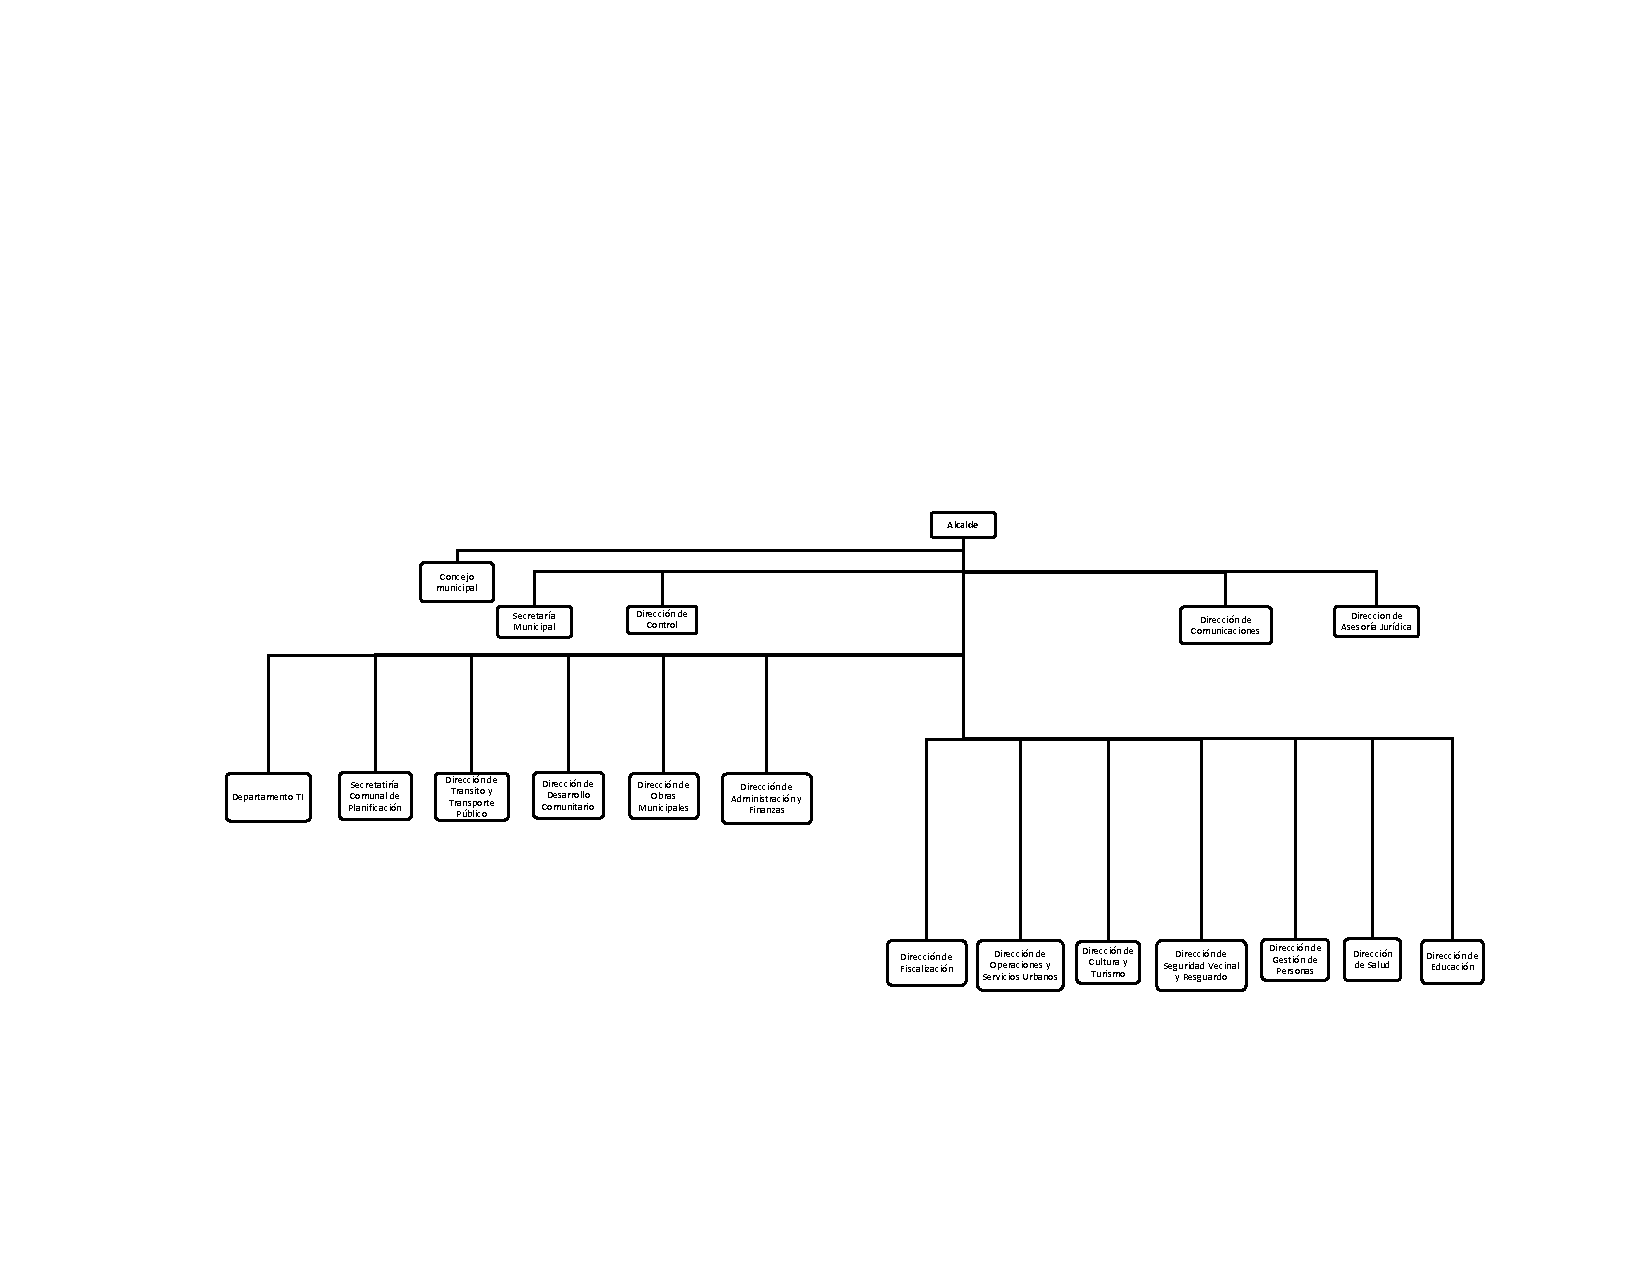
\includegraphics[width=1\textwidth]{fragments/01structure/organigramaMunicipalidad.pdf}\\
\caption{Organigrama}
\label{FIG:ORGANIGRAMA}
\end{figure}


\subsection{Rationale}
El alcance de este trabajo abarca solo las siguientes divisiones:
\begin{itemize}
	\item {
		\textbf{Departamento de asuntos municipales}. Perteneciente a la secretaría municipal. Este se compone de las siguientes oficinas:
		\begin{itemize}
			\item Oficina de partes alcaldía
			\item Sección resolutiva
			\item Sección administrativa
		\end{itemize}
	}
	\item {
		\textbf{Departamento de certificación y archivo}.  Perteneciente a la secretaría municipal. Este se compone de las siguientes oficinas:
		\begin{itemize}
			\item Oficina de registro municipal de transferencias
			\item Oficina de control de archivo y representación.
		\end{itemize}
	}
	\item {
		\textbf{Departamento de cartografía}.
	}
	\item {
		\textbf{Departamento de revisión de procesos de contratación pública}
	}
	\item {
		\textbf{Departamento de auditoría operativa}
	}
	\item {
		\textbf{Departamento Revisión de procesos de pago, bienes y servicios}
	}
\end{itemize}

Se establece para cada departamento la siguiente estructura base:
\begin{itemize}
	\item Un(a) Jefe(a) de departamento.
	\item Un(a) Secretario(a) general de departamento.
	\item Uno o más ejecutivos de departamento.
	\item Un encargado de TI del departamento.
\end{itemize}


Se establece para cada oficina la siguiente estructura base:
\begin{itemize}
	\item Un(a) Jefe(a) de oficina.
	\item Un(a) Secretario(a) general.
	\item Uno o más ejecutivos de oficina.
\end{itemize}

Se establece para cada secretaría la siguiente estructura base:
\begin{itemize}
	\item Un(a) Secretario(a) general.
	\item Uno o más ejecutivos de oficina.
\end{itemize}



\section{Identificación de activos}
Durante la identificación de activos esta se ha limitado a activos que puedan presentar riesgos de seguridad de la información, ignorando los activos humanos y los activos de servicios de TI ya que escapan a situaciones bajo el control directo y supervisión de el equipo de TI. Adicionalmente está especificado en la especificación del proyecto que dichos factores no deben de ser incluidos.

\subsection{Activos de carácter transversal}
A continuación se listan los activos de caracter transversal, quiere decir, cuyo uso se extiende por más de una sola oficina.

\informationResource
{RTR\_PRINC\_001}
{Router principal Cisco 2901, gateway externo perteneciente a la municipalidad}
{Hardware TI}
{Sala de servidores - primer piso}
{Departamento de TI}
{1}{5}{5}
{
	\threatCVE{CVE-2013-1241}{Autenticación inválida en cabeceras del módulo ISM} \\ &
	\threatResourceLost \\ &
	\threatRemoteIntervention \\ &
	\threatNaturalDisaster \\ &
	\threatHumanDisaster \\ &
	\riskNameQuiebreAutenticacionDeTarjetaMagnetica \\ &
	\riskNameFaltaDeMonitoreo
}

\informationResource
{RTR\_SECUN\_001}
{Router secundario Cisco 2901, utilizado de punto intermedio hacia la red interna}
{Hardware TI}
{Sala de servidores - primer piso}
{Departamento de TI}
{1}{5}{5}
{
	\threatCVE{CVE-2017-3881}{Ejecución arbitraria de código (resuelto)} \\ &
	\threatResourceLost \\ &
	\threatRemoteIntervention \\ &
	\threatNaturalDisaster \\ &
	\threatHumanDisaster \\ &
	\riskNameQuiebreAutenticacionDeTarjetaMagnetica \\ &
	\riskNameFaltaDeMonitoreo
}

\informationResource
{SWI\_NODES\_001}
{Switch general Cisco Catalyst 2960, para nodo base del arbol de conectividad}
{Hardware TI}
{Sala de servidores - primer piso}
{Departamento de TI}
{1}{5}{5}
{
	\threatCVE{CVE-2017-3881}{Ejecución arbitraria de código (resuelto)} \\ &
	\threatResourceLost \\ &
	\threatRemoteIntervention \\ &
	\threatNaturalDisaster \\ &
	\threatHumanDisaster \\ &
	\riskNameQuiebreAutenticacionDeTarjetaMagnetica \\ &
	\riskNameFaltaDeMonitoreo
}

\informationResource
{SRV\_SHARE\_001}
{Dell PowerEdge R520 750W E5 2440}
{Hardware TI}
{Sala de servidores - primer piso}
{Departamento de TI}
{5}{5}{5}
{
	\threatRemoteIntervention \\ &
	\threatNaturalDisaster \\ &
	\threatHumanDisaster \\ &
	\riskNameQuiebreAutenticacionDeTarjetaMagnetica \\ &
	\riskNameFaltaDeMonitoreo
	
}


\informationResource
{OSS\_WINDO\_001}
{Windows Server 2019 Datacenter Edition}
{Sistemas Operativos}
{SRV_SHARE_001}
{Departamento de TI}
{2}{5}{5}
{
	Mas de 390 vulnerabilidades detectadas\footnote{https://www.cvedetails.com/product/50662/Microsoft-Windows-Server-2019.html?vendor_id=26} \\ &
	\threatRemoteIntervention \\ &
	\threatLicenceDependant \\ &
	\threatAntivirus
	\riskNameDependenciaDeLicencias \\ &
	\riskNameDesastresLogicos
	\riskNameFaltaDeEncriptado
	\riskNameCarenciaDeLicencias
	\riskNameFaltaDeProtocoloDeBorradoDeInformacion
}


\informationResource
{EXE\_EXCHA\_001}
{Módulo servidor para Microsoft Exchange 2016, para uso de correos corporativos de los funcionarios de la municipalidad.}
{Software}
{SRV_SHARE_001}
{Departamento de TI}
{5}{5}{5}
{
	\threatCVE{CVE-2018-8374}{Tampering Vulnerability existente al momento de un fallo en la información de los perfiles} \\ &
	\threatCVE{CVE-2018-8302}{Ejecución de código remota debido al fallo de manipulación de objetos en memoria, resultante en control total} \\ &
	\threatCVE{CVE-2018-8159}{ XSS resultante en elevación de privilegios por medio de requests web } \\ &
	\threatCVE{CVE-2018-8154}{Ejecución de código remota debido a la corrupción del manejo de objetos en memoria, resultante en control total} \\ &
	\threatCVE{CVE-2018-8153}{ Spoofing } \\ &
	\threatCVE{CVE-2018-8152}{ Elevación de privilegios } \\ &
	\threatCVE{CVE-2018-8151}{ Corrupción de memoria } \\ &
	\threatRemoteIntervention  \\ &
	\riskNameDesastresLogicos \\ &
	\riskNameDependenciaDeLicencias \\ &
	\riskNameFaltaDeEncriptado \\ &
	\riskNameCarenciaDeLicencias \\ &
	\riskNameFaltaDeProtocoloDeBorradoDeInformacion \\ &
	\riskNameRecuperacionDesastres \\ &
	\riskNameRespaldoInexistente \\ & 
	\riskNameFaltaDeDocumentacionEImplantacionDePoliticasParaEnvioDeCorreosMasivos
}

\informationResource
{ARC\_LOCAL\_001}
{Archivo general de la municipalidad - registro de documentos}
{Activos tangibles / Activos intangibles}
{Archivo - Primer piso}
{Departamento de Certificación y Archivos}
{5}{4}{2}
{
	\threatNoPhysicalBackup \\ &
	\threatNoDigitalBackup \\ &
	\threatHumanIntervention \\ &
	\threatNoTransactionRegistry
}

\phpApplicationBaseStructure[appdefinition={
	\informationResource
	{EXE\_WPRES\_001}
	{Servidor Wordpress 5.1 Beta3 para página institucional}
	{Software}
	{SRV\_SHARE\_001}
	{Departamento de TI}
	{1}{3}{3}
	{
		\threatCVE{CVE-2019-9787}{Ejecución remota de código por medio de CRSRF} \\ &
		\threatCVE{CVE-2019-16220}{Sanitización de wp\_validate manipula redirects} \\ &
		\threatHumanIntervention \\ &
		\threatRemoteIntervention
	}
},
apprefr=EXE\_WPRES\_001,
srvrefr=SRV\_SHARE\_001,
dbsrvrefr=EXE\_MYSQL\_001,
dbsrvrefconfi=1,
dbsrvrefinteg=3,
dbsrvrefavail=3,
dbinstrefr=EXE\_SQLTB\_001,
dbinstrefconfi=1,
dbinstrefinteg=3,
dbinstrefavail=3,
dbinstrefcve={
	\threatTransitive
},
phpinstrefr=EXE\_PHPSR\_001,
phpinstrefconfi=1,
phpinstrefinteg=3,
phpinstrefavail=3]{}



\phpApplicationBaseStructure[appdefinition={
	\informationResource
	{EXE\_ADMIN\_002}
	{Servidor con aplicativo de administración propia para municipio}
	{Software}
	{SRV\_SHARE\_002}
	{Departamento de TI}
	{5}{5}{5}
	{
		\threatUnkown \\ &
		\threatTransitive \\ &
		\riskNameRecuperacionDesastres \\ &
		\riskNameRespaldoInexistente \\ &
		\riskNameInteroperabilidadConEstandarInexistente \\ &
		\riskNameTransaccionRota \\ &
		\riskNameFaltaDeEncriptado \\ &
		\riskNameResiduosDeInformacion \\ &
		\riskNameDependenciaDeLicencias \\ &
		\riskNameEjecucionDeMalwareporFaltaDeSoftwareAv \\ &
		\riskNameDenegacionDeServicio \\ &
		\riskNameDesastresHumanos
	}
},
apprefr=EXE\_ADMIN\_002,
srvrefr=SRV\_SHARE\_002,
dbsrvrefr=EXE\_MYSQL\_002,
dbsrvrefconfi=4,
dbsrvrefinteg=5,
dbsrvrefavail=4,
dbinstrefr=EXE\_SQLTB\_002,
dbinstrefconfi=5,
dbinstrefinteg=5,
dbinstrefavail=5,
dbinstrefcve={
	\threatTransitive
	
},
phpinstrefr=EXE\_PHPSR\_002,
phpinstrefconfi=4,
phpinstrefinteg=5,
phpinstrefavail=4]{}


\phpApplicationBaseStructure[appdefinition={
	\informationResource
	{EXE\_ADMIN\_003}
	{Servidor con aplicativo de administración para archivo de municipio}
	{Software}
	{SRV\_SHARE\_003}
	{Departamento de TI}
	{5}{5}{5}
	{
		\threatUnkown \\ &
		\threatTransitive \\ &
		\riskNameQuiebreAutenticacionDeLlaveSeguridad \\ &
		\riskNameFaltaDeEncriptado \\ &
		\riskNameDependenciaDeLicencias \\ &
		\riskNameFaltaDeProtocoloDeBorradoDeInformacion
		
	}
},
apprefr=EXE\_ADMIN\_003,
srvrefr=SRV\_SHARE\_003,
dbsrvrefr=EXE\_MYSQL\_003,
dbsrvrefconfi=4,
dbsrvrefinteg=5,
dbsrvrefavail=4,
dbinstrefr=EXE\_SQLTB\_003,
dbinstrefconfi=5,
dbinstrefinteg=5,
dbinstrefavail=5,
dbinstrefcve={
	\threatTransitive
	
},
phpinstrefr=EXE\_PHPSR\_003,
phpinstrefconfi=4,
phpinstrefinteg=5,
phpinstrefavail=4]{}




\subsection{Activos de carácter específico}
A continuación se listan los activos de caracter específico, quiere decir, cuyo uso es solo de un oficina, departamento o sección en particular.

\subsubsection{Oficina de Partes Alcaldía}
\repeatOnEachOfficeBase{OF001}{Oficina de Partes Alcaldía}{Departamento de Asuntos Municipales}

\subsubsection{Oficina de Registro Municipal de Transferencias}
\repeatOnEachOfficeBase{OF002}{Oficina de Registro Municipal de Transferencias}{Departamento de Certificación y Archivo}

\subsubsection{Oficina de Control de Archivo y reorsentación}
\repeatOnEachOfficeBase{OF003}{Oficina de Control de Archivo y reorsentación}{Departamento de certificación y archivo}

\subsubsection{Sección Resolutiva}
\repeatOnEachSecretaryBase{SE001}{Sección Resolutiva}{Departamento de Asuntos Municipales}

\subsubsection{Sección Administrativa}
\repeatOnEachSecretaryBase{SE002}{Sección Administrativa}{Departamento de Asuntos Municipales}

\subsubsection{Departamento de Asuntos Municipales}
\repeatOnEachDepartmentBase{DP001}{Departamento de Asuntos Municipales}{primer piso}

\subsubsection{Departamento de Certificación y archivo}
\repeatOnEachDepartmentBase{DP002}{Departamento de Certificación y Archivo}{segundo piso}

\subsubsection{Departamento de Cartografía }
\repeatOnEachDepartmentBase{DP003}{Departamento de Cartografía}{tercer piso}

\subsubsection{Departamento de Revisión de Procesos de Contratación }
\repeatOnEachDepartmentBase{DP004}{Departamento de Revisión de Procesos de Contratación Pública}{cuarto piso}

\subsubsection{Departamento de Auditoría Operativa}
\repeatOnEachDepartmentBase{DP005}{Departamento de Auditoría Operativa} {quinto piso}

\subsubsection{Dirección de revisión de Procesos de Pago, Bienes y Servicios}
\repeatOnEachDepartmentBase{PP001}{Dirección de Desarrollo Comunitario} {sexto piso}

\subsubsection{Departamento de Tecnologías de la Información}
\repeatOnEachDepartmentBase{TI001}{Departamento de Tecnologías de la Información} {primer piso}



\section{Análisis de riesgos}
%% dependencies
%% Approbal 
\newcommand{\riskPOIAsuntosMunicipales}{
	Jefe de Oficina de Asuntos Municipales.
}
\newcommand{\riskPOIConsejoMunicipal}{
	Jefe de Consejo municipal.
}
\newcommand{\riskPOISecretariaMunicipal}{
	Jefe de Secretaría Municipal
}
\newcommand{\riskPOIDireccionControl}{
	Jefe de Dirección de Control.
}
\newcommand{\riskPOIDireccionComunicaciones}{
	Jefe de Dirección de Comunicaciones.
}
\newcommand{\riskPOIDireccionAsistenciaJuridica}{
	Jefe de Dirección de Asesoría Jurídica.
}
\newcommand{\riskPOIDepartamentoTecnologias}{
	Jefe de Departamento de Tecnologías de la Información.
}
\newcommand{\riskPOISecretariaComunalDePlanificacion}{
	Jefe de Secretaría Comunal de Planificación.
}
\newcommand{\riskPOIDireccionTransitoTransportePublico}{
	Jefe de Dirección de Tránsito y Transporte Público.|
}
\newcommand{\riskPOIDesarolloComunitario}{
	Jefe de Dirección de Desarrollo Comunitario
}
\newcommand{\riskPOIDireccionObrasMunicipales}{
	Jefe de Dirección de Obras Municipales
}
\newcommand{\riskPOIDireccionAdministracionFinanzas}{
	Jefe de Dirección de Administración y Finanzas
}
\newcommand{\riskPOIDireccionFiscalizacion}{
	Jefe de Dirección de Fiscalización
}
\newcommand{\riskPOIDireccionDeOperaciones}{
	Jefe de Dirección de Operaciones y Servicios Urbanos
}
\newcommand{\riskPOIDireccionCulturaTurismo}{
	Jefe de Dirección de Cultura y Turismo
}
\newcommand{\riskPOIDireccionSeguridadVecinal}{
	Jefe de Dirección de Seguridad Vecinal y Resguardo
}
\newcommand{\riskPOIDireccionGestionPersonas}{
	Jefe de Dirección de Gestión de Personas
}
\newcommand{\riskPOIDireccionSalud}{
	Jefe de Dirección de Salud
}
\newcommand{\riskPOIDireccionEducacion}{
	Jefe de Dirección de Educación
}
\newcommand{\riskPOIEmpresaExterna1}{
	Empresa Externa 1
}
\newcommand{\riskPOIEmpresaExterna2}{
	Empresa Externa 2
}
\newcommand{\riskPOIEmpresaExterna3}{
	Empresa Externa 3
}
\newcommand{\riskPOIEmpresasExternas}{
	Empresas externas
}
\newcommand{\riskPOIAlcalde}{
	Alcalde
}
\newcommand{\riskPOIGeneral}{
	Dominio General
}
\newcommand{\riskPOIArchivo}{
	Jefe de Departamento de Certificación y Archivo
}

\newcommand{\riskPOIDepartamentoTecnologias}{
	Jefe de Departamento de Tecnologías de la Información.
}
\newcommand{\riskPOICartografia}{
	Jefe de Departamento de cartografía
}

\newcommand{\riskPOIAuditoria}{
	Jefe de Departamento de auditoria operativa
}
\newcommand{\riskPOIPago}{
	Jefe de Departamento revisión de procesos de pago, bienes y servicios
}

\newcommand{\riskPoiRevisionProcesos}{
	Jefe de Departamento de revisión de procesos de contratación pública
}


%% Authors
\newcommand{\riskAuthorErik}{
	Erik Regla
}\newcommand{\riskAuthorAriel}{
	Ariel Valenzuela
}\newcommand{\riskAuthorMiguel}{
	Miguel Jorquera
}

%% Response 
\newcommand{\riskRepsonsePrevent}{
	PREVENIR
}\newcommand{\riskRepsonseMitigate}{
	MITIGAR
}\newcommand{\riskRepsonseCorrect}{
	CORREGIR
}\newcommand{\riskRepsonseCompensate}{
	COMPENSAR
}\newcommand{\riskRepsonseTransfer}{
	TRANSFERIR
}

%% Processes 
\newcommand{\riskProcessGetAppointment}{
	Obtención de hora de atención.
}\newcommand{\riskProcessNewSuggestion}{
	Entrega de sugerencias.
}\newcommand{\riskProcessNewClaim}{
	Entrega de reclamos.
}\newcommand{\riskProcessGetInformation}{
	Solicitud de información.
}\newcommand{\riskProcessUsoDeSitioWeb}{
	Disponibilidad sitio web.
}\newcommand{\riskProcessConfiabilidadDeSitioWeb}{
	Confiabilidad sitio web.
}\newcommand{\riskProcessResguardoInformacionPersonal}{
	Resguardo de información personal.
}\newcommand{\riskProcessResguardoInformacionInstitucional}{
	Resguardo de información institucional.
}

\makeatletter
\define@key{riskItem}{riskTitle}{\def\risk@riskTitle{#1}}
\define@key{riskItem}{riskAuthor}{\def\risk@riskAuthor{#1}}
\define@key{riskItem}{riskDate}{\def\risk@riskDate{#1}}
\define@key{riskItem}{riskDescription}{\def\risk@riskDescription{#1}}
\define@key{riskItem}{riskResourceOwner}{\def\risk@riskResourceOwner{#1}}
\define@key{riskItem}{riskAssociatedProcess}{\def\risk@riskAssociatedProcess{#1}}
\define@key{riskItem}{riskSubArea}{\def\risk@riskSubArea{#1}}
\define@key{riskItem}{riskSubAreaDependencies}{\def\risk@riskSubAreaDependencies{#1}}
\define@key{riskItem}{riskVulnDetails}{\def\risk@riskVulnDetails{#1}}
\define@key{riskItem}{riskThreatDetails}{\def\risk@riskThreatDetails{#1}}
\define@key{riskItem}{riskResponse}{\def\risk@riskResponse{#1}}
\define@key{riskItem}{riskApproval}{\def\risk@riskApproval{#1}}

\setkeys{riskItem}{
riskTitle=riskTitle,
riskAuthor=riskAuthor,
riskDate=riskDate,
riskDescription=riskDescription,
riskResourceOwner=riskResourceOwner,
riskAssociatedProcess=riskAssociatedProcess,
riskSubArea=riskSubArea,
riskSubAreaDependencies=riskSubAreaDependencies,
riskVulnDetails=riskVulnDetails,
riskThreatDetails=riskThreatDetails,
riskResponse=riskResponse,
riskApproval=riskApproval
}

\newcommand{\riskItemTable}[2][]{%
    \setkeys{riskItem}{#1}% Set the keys

    \begin{tabularx}{\linewidth}{|r|X|}
        \hline
        \textbf{Título de Riesgo}      & \risk@riskTitle  \\ 
        \hline
        \textbf{Autor} & \risk@riskAuthor  \\ 
        \hline
        \textbf{Fecha de Levantamiento}   & \risk@riskDate  \\ 
        \hline
        \textbf{Descripción}   & \risk@riskDescription  \\ 
        \hline
        \textbf{Dueño del Activo} & \risk@riskResourceOwner  \\ 
        \hline
        \textbf{Proceso}      & \risk@riskAssociatedProcess  \\ 
        \hline
        \textbf{Sub Área} & \risk@riskSubArea  \\ 
        \hline
        \textbf{Dependencia}   & \risk@riskSubAreaDependencies  \\ 
        \hline
        \textbf{Detalle de la Vulnerabilidad}   & \risk@riskVulnDetails  \\ 
        \hline
        \textbf{Detalle de la amenaza} & \risk@riskThreatDetails  \\ 
        \hline
        \textbf{Respuesta}   & \risk@riskResponse  \\ 
        \hline
        \textbf{Aprobación} & \risk@riskApproval  \\ 
        \hline
        %\textbf{Valoración}  &  \makecell[l]{Confidencialidad: #6\\ Integridad: #7\\ Disponibilidad: #8}\\
        %\hline
        %\textbf{\makecell[r]{Vulnerabilidades y \\Amenazas}}  &  \makecell[l]{#9}\\ 
        %\hline
    \end{tabularx}
    #2
}

\makeatother
%% SubAreas y dependencias
\newcommand{\riskSubAreaAsuntosMunicipales}{
	Departamento de Asuntos Municipales.
}
\newcommand{\riskSubAreaArchivo}{
	Departamento de Certificación y Archivo
}

\newcommand{\riskSubAreaDepartamentoTecnologias}{
	Departamento de Tecnologías de la Información.
}
\newcommand{\riskSubAreaCartografia}{
	Departamento de cartografía
}
\newcommand{\riskSubAreaRevisionProcesos}{
	Departamento de revisión de procesos de contratación pública
}
\newcommand{\riskSubAreaAuditoria}{
	Departamento de auditoria operativa
}
\newcommand{\riskSubAreaPago}{
	Departamento revisión de procesos de pago, bienes y servicios
}
\newcommand{\riskSubAreaNone}{
	Ninguna.
}
\newcommand{\riskSubAreaAll}{
	Todas.
}
\newcommand{\riskSubAreaMajor}{
	Alcalde.
}

%%Begin of content

\section{Riesgos asociados a la atención de público}
\riskItemTable[
    riskTitle={Imposibilidad de obtener una hora de atención a público},
    riskAuthor={\riskAuthorErik},
    riskDate={11/06/2020},
    riskDescription={
        Al materializarse este riesgo, una persona natural
        queda imposibilitada de poder solicitar una hora para su atención, 
        lo cual genera un cuello de botella.},
    riskResourceOwner={\riskPOIAsuntosMunicipales},
    riskAssociatedProcess={
        \riskProcessGetAppointment  \\&
        \riskProcessNewSuggestion   \\&
        \riskProcessNewClaim        \\&
        \riskProcessGetInformation
    },
    riskSubArea={ \riskSubAreaOIRS },
    riskSubAreaDependencies={ \riskSubAreaAsuntosMunicipales },
    riskVulnDetails={
        Bla bla bla, el programa utilizado en bla bla...
        
        Debido a que la versión del sistema operativo utilizado tiene una gran cantidad de CVEs activos, existe la posibilidad de que un usuario malicioso intente generar un ataque de denegación de servicio dentro de la misma municipalidad.
    },
    riskThreatDetails={
        Bla bla bla, el programa utilizado en bla bla...
        
        Debido a que la versión del sistema operativo utilizado tiene una gran cantidad de CVEs activos, existe la posibilidad de que un usuario malicioso intente generar un ataque de denegación de servicio dentro de la misma municipalidad.
    },
    riskResponse={ \riskRepsonsePrevent },
    riskApproval={ \riskPOIAsuntosMunicipales }
]{}

\section{Riesgos asociados a plataformas o tecnologías generalizados dentro de la organización}

\riskItemTable[
    riskTitle={Denegación de servicio},
    riskAuthor={\riskAuthorErik},
    riskDate={11/06/2020},
    riskDescription={
        Al materializarse este riesgo, el sitio web de la municipalidad deja de quedar disponible para todo público.},
    riskResourceOwner={\riskPOIDepartamentoTecnologias},
    riskAssociatedProcess={
        Nivel general, \riskProcessUsoDeSitioWeb
    },
    riskSubArea={ 
        \riskSubAreaDireccionComunicaciones \\&
        \riskSubAreaAsuntosMunicipales      \\&
        \riskSubAreaDepartamentoTecnologias 
    },
    riskSubAreaDependencies={ \riskPOIDepartamentoTecnologias  },
    riskVulnDetails={
        La denegación de servicio es un tipo de ataque cuyo fin es eliminar temporal o parcialmente la disponibilidad de un servicio, usualmente por medios como ICMP Flood.
    },
    riskThreatDetails={
        Si bien la aplicación está funcionando con las últimas versiones de PHP y de MYQSL disponibles, la infraestructura al ser local y no contar con un WAF, no hay filtro respecto a las peticiones que son resueltas en el servidor. Debido a esto, en caso de llegar un número importante de peticiones las cuales no pudiesen resolverse simultaneamente, podría ocurrir un problema de overflow de memoria colapsando el proceso.

        Cabe destacar que esto también puede ocurrir de manera orgánica en situaciones de alta demanda. Y debido a los acuerdos internos de desarrollo estandarizado, está presente en todas las plataformas desarolladas para uso interno.
    },
    riskResponse={ \riskRepsonseCorrect },
    riskApproval={ \riskPOIDepartamentoTecnologias }
]{}


\riskItemTable[
    riskTitle={Ejecución remota de código},
    riskAuthor={\riskAuthorErik},
    riskDate={11/06/2020},
    riskDescription={
        Al materializarse este riesgo, el atacante ejecuta código en el navegador del cliente sin previo consentimiento.},
    riskResourceOwner={\riskPOIDepartamentoTecnologias},
    riskAssociatedProcess={
        Nivel general, \riskProcessUsoDeSitioWeb
        % \threatInterest \\&
        % \threatHumanIntervention
    },
    riskSubArea={ 
        \riskSubAreaAll
    },
    riskSubAreaDependencies={ \riskPOIDepartamentoTecnologias  },
    riskVulnDetails={
        La ejecución remota de código permite que un usuario no autorizado ejecute instrucciones en otro equipo.
    },
    riskThreatDetails={
        Esta amenaza está atribuida a CVE-2019-9787, el cual especifica una vulnerabilidad sobre la ejecución remota de código por medio de CRSRF. Este tipo de ataque fuerza al usuario a ejecutar código utilizando sus credenciales ya cargadas en la aplicación.
    },
    riskResponse={ \riskRepsonsePrevent },
    riskApproval={ \riskPOIDepartamentoTecnologias }
]{}

\riskItemTable[
    riskTitle={Manipulación de redirecciones},
    riskAuthor={\riskAuthorErik},
    riskDate={11/06/2020},
    riskDescription={
        Al materializarse este riesgo, el atacante fuerza la redirección a un sitio externo.},
    riskResourceOwner={\riskPOIDepartamentoTecnologias},
    riskAssociatedProcess={
        Nivel general, \riskProcessUsoDeSitioWeb \\&
        Nivel general, \riskProcessConfiabilidadDeSitioWeb
    },
    riskSubArea={ 
        \riskSubAreaAll
    },
    riskSubAreaDependencies={ \riskPOIDepartamentoTecnologias  },
    riskVulnDetails={
        La ejecución remota de código permite que un usuario no autorizado ejecute instrucciones en otro equipo.
    },
    riskThreatDetails={
        Esta amenaza está atribuida a CVE-2019-16220, el cual especifica una vulnerabilidad sobre la ejecución remota de código por medio de CRSRF. Este tipo de ataque fuerza al usuario a ejecutar código utilizando sus credenciales ya cargadas en la aplicación.
    },
    riskResponse={ \riskRepsonseMitigate },
    riskApproval={ \riskPOIDepartamentoTecnologias }
]{}


\riskItemTable[
    riskTitle={Ejecución de malware en servidor principal},
    riskAuthor={\riskAuthorErik},
    riskDate={11/06/2020},
    riskDescription={
        Al materializarse este riesgo, el servidor principal de la municipalidad queda comprometido.},
    riskResourceOwner={\riskPOIDepartamentoTecnologias},
    riskAssociatedProcess={
    },
    riskSubArea={ 
        \riskSubAreaAll
    },
    riskSubAreaDependencies={ \riskPOIDepartamentoTecnologias  },
    riskVulnDetails={
        Ataques por randomware, gusanos, trojanos, etc.
    },
    riskThreatDetails={
        Debido al alto número de vulnerabilidades presentes en el sistema operativo, es posible que la materalización de un riesgo en un equipo de una red adyacente pueda propagar procesos de terceros y estos comprometan el servidor principal.
    },
    riskResponse={ \riskRepsonsePrevent },
    riskApproval={ \riskPOIDepartamentoTecnologias }
]{}


\section{Riesgos generales asociados a ingenería social}

\riskItemTable[
    riskTitle={Phishing},
    riskAuthor={\riskAuthorErik},
    riskDate={11/06/2020},
    riskDescription={
        Al materializarse este riesgo, un usuario ingresa información institucional a un sitio falso.},
    riskResourceOwner={\riskPOIDepartamentoTecnologias},
    riskAssociatedProcess={
    },
    riskSubArea={ 
        \riskSubAreaAll
    },
    riskSubAreaDependencies={ \riskPOIDepartamentoTecnologias  },
    riskVulnDetails={
        Un usuario recibe un correo con un mensaje falso pero con apariencia visual creible, de esta manera para tentar al usuario a ejecutar alguna acción que pueda comprometer la seguridad, ya sea filtrando credenciales o información sensible.
    },
    riskThreatDetails={
        Un ataque de Phishing implica la personificación de otro individuo o entidad, la cual actua como emisor de un mensaje el cual puede ser de interés del usuario. En este caso la apuesta es que el lector del correo hará caso del call to action antes de verificar la veracidad del contenido, por lo que este tipo de ataques está dirigido a un público no tecnico.
    },
    riskResponse={ \riskRepsonsePrevent },
    riskApproval={ \riskPOIDepartamentoTecnologias }
]{}



\section{Riesgos generales asociados a activos estándares}


\section{Matriz de riesgos}
\section{Política de seguridad}


\begin{thebibliography}{9}
% 	\bibitem{REF:crc}
% 	Bill McDaniel.
% 	\textit{An Algorithm for Error Correcting Cyclic Redundance Checks}.
% 	https://www.drdobbs.com/an-algorithm-for-error-correcting-cyclic/184401662, 2002.

% 	\bibitem{REF:gnupg}
% 	Linux Man pages.
% 	\textit{gpg(1) - Linux man page}.
% 	https://linux.die.net/man/1/gpg.


% 	\bibitem{REF:veracrypt}
% 	VeraCrypt.
% 	\textit{Documentation}.
% 	https://www.veracrypt.fr/en/Documentation.html.


% 	\bibitem{REF:mellon}
% 	Koopman, Philip and Chakravarty, T.
% 	\textit{Cyclic redundancy code (CRC) polynomial selection for embedded networks}.
% 	10.1109/DSN.2004.1311885. 2004.


\end{thebibliography}

\end{document}